% This is samplepaper.tex, a sample chapter demonstrating the
% LLNCS macro package for Springer Computer Science proceedings;
% Version 2.20 of 2017/10/04
%
\documentclass[runningheads]{llncs}
%
\usepackage[T1]{fontenc}
\usepackage{graphicx}
\graphicspath{{img/}}
% Used for displaying a sample figure. If possible, figure files should
% be included in EPS format.
%
% If you use the hyperref package, please uncomment the following line
% to display URLs in blue roman font according to Springer's eBook style:
\usepackage{hyperref,xcolor}
\renewcommand\UrlFont{\color{blue}\rmfamily}

\usepackage{fancyvrb}

\usepackage{url}
\urldef{\mailsa}\path|amrendonsa@unal.edu.co|  

\begin{document}
%
\title{Proposal for Blockchain-Based Applications Architecture, Case of Study: Electronic Certification System}
%
\titlerunning{Blockchain-Based Applications Proposal Architecture}
% If the paper title is too long for the running head, you can set
% an abbreviated paper title here
%
\author{Angel Rendon\orcidID{0000-0003-3900-9582}}
%
%\authorrunning{A. Rendon et al.}
% First names are abbreviated in the running head.
% If there are more than two authors, 'et al.' is used.
%
\institute{
Universidad Nacional de Colombia\\
\mailsa\\
\url{http://unal.edu.co/}
}
%
\maketitle              % typeset the header of the contribution
%
\begin{abstract}
Blockchain has become an appealing technology for the software industry as the SmartContracts appeared as another of its applications alongside to cryptocurrencies. Technologies such as the Ethereum Virtual Machine (EVM) have opened a whole new landscape for developers to come up with more efficient solutions taking advantage of its qualities (e.g., decentralization, transparency, traceability, auditability, etc).

As the technology gains a more important role, a need for having a set of good practices rises as key element in software development.

This paper aims to explore topics that motivates this work: what has been done at the architectural side, as well as showing our own experience exploring the development of a blockchain certification tool for Universidad Nacional de Colombia's Engineering Faculty extension courses diplomas, using Solidity, deploying the SmartContract to the Ropsten test net (including the tools used for such purpose), and integrating it into a microservices architecture for our architecture proposal.

At the end, this paper will briefly show what are the next stages for the project under analysis and conclusions.

\keywords{Blockchain \and Software architecture \and Applications \and Architectural views.}
\end{abstract}
%

\section{Introduction}


\section{Related work}

The very essence of a certification lies on issuing a statement from certain party to any other else that a set of facts are actually veracious. In a normal certification process there is a \textbf{claim} emited by an \textbf{issuer} based on \textbf{evidences} about a \textbf{recipient} (i.e., the entity that is being certified) by means of a \textbf{certificate} as a document that attest all of them: the issuer, the recipient, the claims upon evidences as needed \cite{grech2017blockchain}.

There are three processes involved on certifying \cite{grech2017blockchain}:
\begin{enumerate}
	\item \textbf{Issuing}: the process where the issuer emits claims based on evidences about a recipient in form of the certificate itself.
	\item \textbf{Sharing}: the process where the recipient shares their certificate with any third-party.
	\item \textbf{Verification}: the process where any third-party verifies the authenticity of a certificate.
\end{enumerate}

However there must be guarantee of having certifications issued by significant trusted parties. Thus, identification of the parties involved gets more importance because third-parties must be able to corroborate by any means such identities \cite{grech2017blockchain}.

Among the advantages of using blockchain for digital certification there are \cite{grech2017blockchain}:
\begin{itemize}
	\item Verification can be done by anyone with access to the blockchain.
	\item Certifications will be still valid even if the original issuer no longer exists.
	\item The only way to lose the certificate information is having all the nodes of the blockchain to delete the network client.
	\item There are mechanisms to share the signature of the document without sharing the document itself
\end{itemize}

As an emerging technology, blockchain is still on early stages of development. There are no well defined design patterns to integrate it into formal developments yet. By replacing central databases with blockchain, it has been demostrated that data structuration on SmartContracts can affect systems' resilience \cite{Xu2019}.

In \cite{Xu2019} a restructured architecture comprised of four layers (i.e., UI; management; data, or off-chain; and, blockchain, or on-chain) was proposed in order to reflect the traceability process of their use case. The key element is to identify where specific data must be placed (i.e., off-chain or on-chain), for that specific case, sensitive information was placed on-chain (e.g., hashes of documents, small and sensitive information, permission control information), whereas off-chain was left with SmartContracts' addresses, and heavy information (e.g., photos, certificates, even SmartContracts' code).

An esential feature in \cite{Xu2019} is the concept of the \emph{factory contract}, that creates, upon certain parameters, different instances of new SmartContracts on-chain. It also avoids modifications on SmartContracts by unauthorized entities.

Due to several configurations and variants systems can adopt depending on the chosen Blockchain technology, \cite{Xu2017} proposes a Blockchain Taxonomy in order to classify and compare different blockchain technologies as a support tool to design and assess their impact on software architectures.

Other natural factors of current blockchains (e.g., decentralization, execution calls delays) as well as external factors such as the way users interact with those blockchains, poses high challenges on integrating blockchain to software developments. By means of surveying several \DH apps \footnote{\DH\ is a glyph used in Old English, Middle English, Faroese, Icelandic and Elfdalian (\url{https://en.wikipedia.org/wiki/Eth}). Its pronuntiation would be something like \emph{eth}. In the Etherum context it has been used to refer decentralized applications or ``Eth-apps'', but many people simply pronounce it like ``Dapps''.}, \cite{Wessling2018} examines their architecture in order to find reocurring architectural patterns.

BSeIn is presented as a conceptual framework \cite{Lin2018} to implement reconfigurable smart factories. This framework aims to enforce fine-grained access control policies to secure several authentications. The design of the framework includes Initialization (where the factory manager or a suitable authority initializes the system upon system paramenters), Request Issuance (proving user can publish a reasonable request, generating key pair, encrypting and signing info, broadcasting transaction to the blockchain), Chain Transaction, State Delivery (transactions are broadcasted to the cloud and industrial networks), and Permission Update.

A comparison for computational and storage cost between blockchains and databases was done in \cite{Rimba2017}, by, first, capturing the cost models for both technologies, and second, implementing and measuring the cost of business process execution on both for a specific use case. As result of this investigation, they have conclude that using blockchain affects non-functional qualities of a system with two orders of magnitude of difference between both aproaches. However, this research only focuses on monetary costs losing the decentralization purpose of blockchain.

Other aproaches explore architectures to share information on ledgers with the government as a way to ensure public safety and security. The purpose on \cite{Engelenburg2017} is to devise the requirements and architecture for information sharing between corporations and goverment so it is acceptable to businesses, by implementing a blockchain solution to store events and rules for information shared by companies by cryptographic means. As key elements some considerations have to be ensured, due to communication between Business and Goverment should be a must, as public safety and security. This article attemps to provide a modern solution by desingning and building an architecture such that:
\begin{itemize}
	\item keeps information confidential between parties
	\item its Reliable
	\item its Secure
	\item allows Goverment to keep track for ``suspicious'' goods
\end{itemize}

Possible outcomes or expected results of this implementations are related mainly with reduction of smuggling and detect whether goods need inspection or not \cite{Engelenburg2017}.

Current software development paradigms have to deal with centralization and their associated problems (i.e., flexibility, efficiency, availability, and security). By integrating blockchain to come up with a P2P network with higher security, scalability and a well-structured cloud system, a system comprised of five layers is presented: resource (physical manufacturing resources), perception (senses physical manufacturing resources), manufacturing (service provider, data hashing service, conection provider), infrastructure (other layers infrastructure supporter) and application (API\footnote{Application Programming Interface} provider) \cite{Li2018c}.

\section{Case of study: Electronic Certification System}
\subsection{Background}
The Engineering Faculty of Universidad Nacional de Colombia proposed a proof of concept project, through the IEI (Instituto de Extensi\'{o}n e Investigaci\'{o}n)\footnote{Research and Extension Institute} associated to the same Faculty, to check the viability of applying the blockchain technology to the certification process.

The first stage of the project considers having a system able to:
\begin{itemize}
	\item generate the certificates on PDF including a QRCode, thus enabling any third-party to verify the metadata in the associated site.
	\item enable any third-party to verify the authenticity of a copy of the PDF in the associated site.
	\item allow University's designed officials to upload a list of students to certify with the according course information.
	\item notify the students to their personal email addresses attaching the PDF certificate, a link to their information, the QRCode, and the PDF certificate hash.
\end{itemize}

The office in charge of certifying the students, La Unidad de Educaci\'{o}n Continua y Permanente\footnote{Permanent and Continuous Education Unit}, has several formats and types of courses. The idea was to focus on a single type of course with its respective certification format, and prove the concept in one of the Unit courses. The decision was finally to certify the course `Blockchain - Creaci\'{o}n de Contratos Inteligentes'\footnote{Blockchain - Creation of Smart Contracts}. This course has a duration of 45 hours distributed on sessions of three hours per day, three sessions per week, for a total of 5 weeks. The course is approved with the 80\% of attendance, it does mean 12 of 15 sessions.

\subsection{Global architecture}
The resulting architecture is shown in Figure~\ref{fig1}. There is a service component of the solution provided by \emph{Infura}. It might be considered as a Decentralized Gateway as a Service, because Infura\footnote{\url{https://infura.io/about}} provides access to the IPFS\footnote{InterPlanetary File System \url{https://docs.ipfs.io/introduction/overview/}} public gateways and Ethereum APIs. Through Infura, it is possible to access all the available Ethereum networks (i.e., MainNet, and Testing networks), the Figure \ref{fig1} only shows Ropsten, because the SmartContract was deployed there.

\begin{figure}
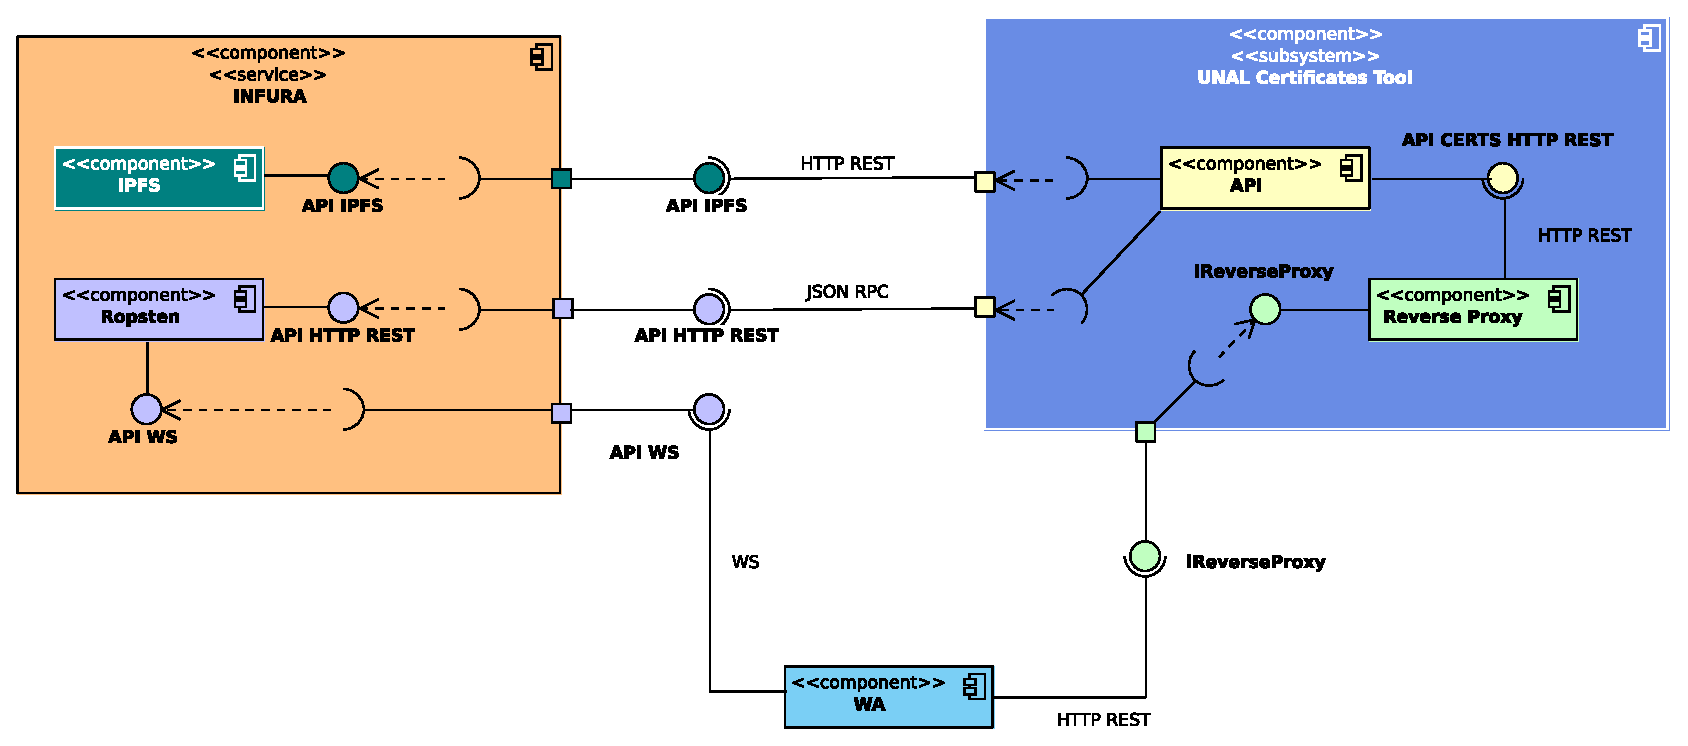
\includegraphics[width=\textwidth]{01-components.eps}
\caption{Microservices architecture for the certifying system.}
\label{fig1}
\end{figure}

The solution is encapsulated into the \emph{UNAL Certificates Tool} subsystem, comprised of the backbone API and a Reverse Proxy. The API is the main component in the architecture because it has the business logic and configurations to interact with the Infura service. The Reverse Proxy uses Nginx in a special configuration, so as to filter certain HTTP requests.

Finally, there is a client \emph{WA} (Web Application) that connects to the API through the Reverse Proxy, and the Ropsten network using the WebSocket protocol in order to track certain transactions on the Blockchain. This is the client used by any third-party to verify certificates' authenticity. It also allows the designated University's officials to fulfill metadata of the course and upload the list of students to be certified.

\subsubsection{WA}
The WA was developed using VueJS (\url{https://vuejs.org/}) as framework. It got the axios (\url{https://github.com/axios/axios}) library to perform HTTP requests to the API through the Reverse Proxy. It also got the web3.js (\url{https://web3js.readthedocs.io/en/1.0/}) library collection to communicate against Ropsten using the IPC communication protocol.

\subsubsection{Reverse Proxy}
A Nginx configuration script running on a Docker container.

\subsubsection{API}
The API is the most important component in the whole architecture scheme. It has the business logic and certain configurations. It was written in JavaScript with Babel (\url{https://babeljs.io/}) integrating Swagger (\url{https://swagger.io/}) in order to expose routes as documentation. For communication effects against the Ethereum's Ropsten network, it got the web3.js (\url{https://web3js.readthedocs.io/en/1.0/}) library collection.

It has three main modules as it can be seen on Figure~\ref{fig2}, the \emph{Sessions} for session handling, \emph{Mailer} for mail construction and transport, and \emph{Certificates} that does all the heavy work on certifying students, the last one uses a series of helpers, such as the \emph{IPFS} which handles all the IPFS operations, \emph{SmartContracts} which interacts through the SmartContract's ABI\footnote{Application Binary Interface} with the deployed SmartContract on the Ropsten network, \emph{PDFBuilder} which makes the actual PDF file on JS Buffers, and \emph{QRCodeBuilder} that makes QRCodes upon a given text.

\begin{figure}
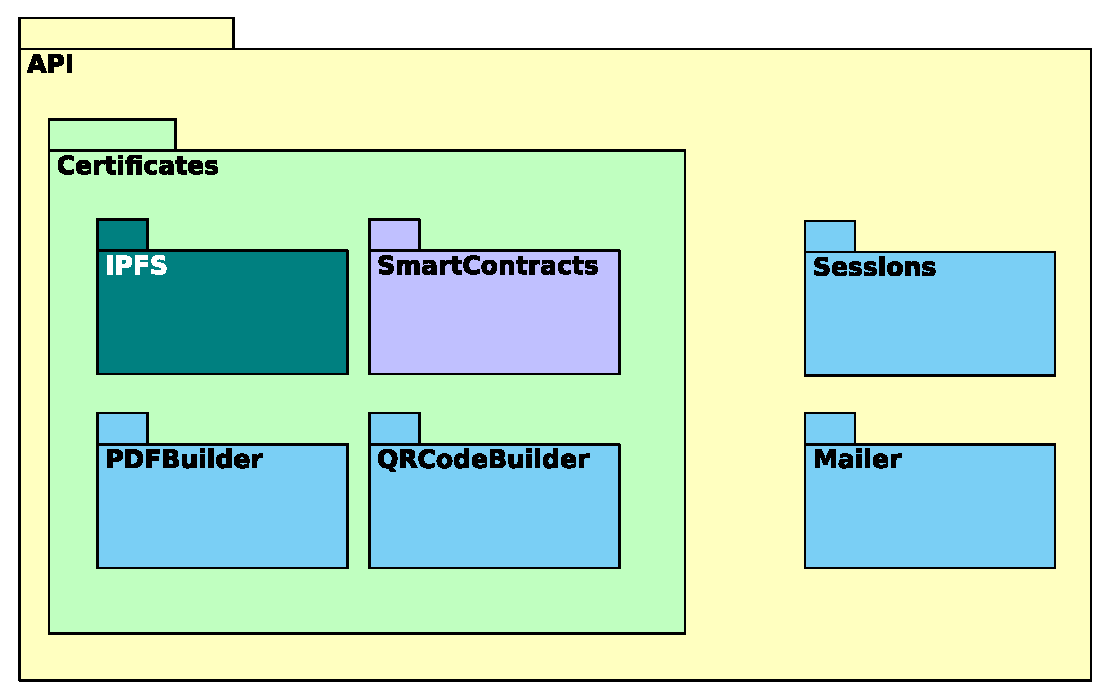
\includegraphics[width=\textwidth]{02-API-Decomposition.eps}
\caption{API decomposition architectural view}
\label{fig2}
\end{figure}

This API was built using ExpressJS (\url{https://expressjs.com/}) as base middleware, allowing to build the solution with a n-tier architecture as shown on Figure~\ref{fig3}. The API has a sequence for valid requests where \emph{Controllers} deal with the initial request, validating authorized operations, the flow goes to the \emph{Services}, where the business logic is coded. The service can request actions from the \emph{Repositories}, where specific configurations are coded for the IPFS and Ropsten networks. The \emph{SmartContract Repository} can access the \emph{Contracts} layer in order to read the compiled SmartContract, specifically its ABI.

\begin{figure}
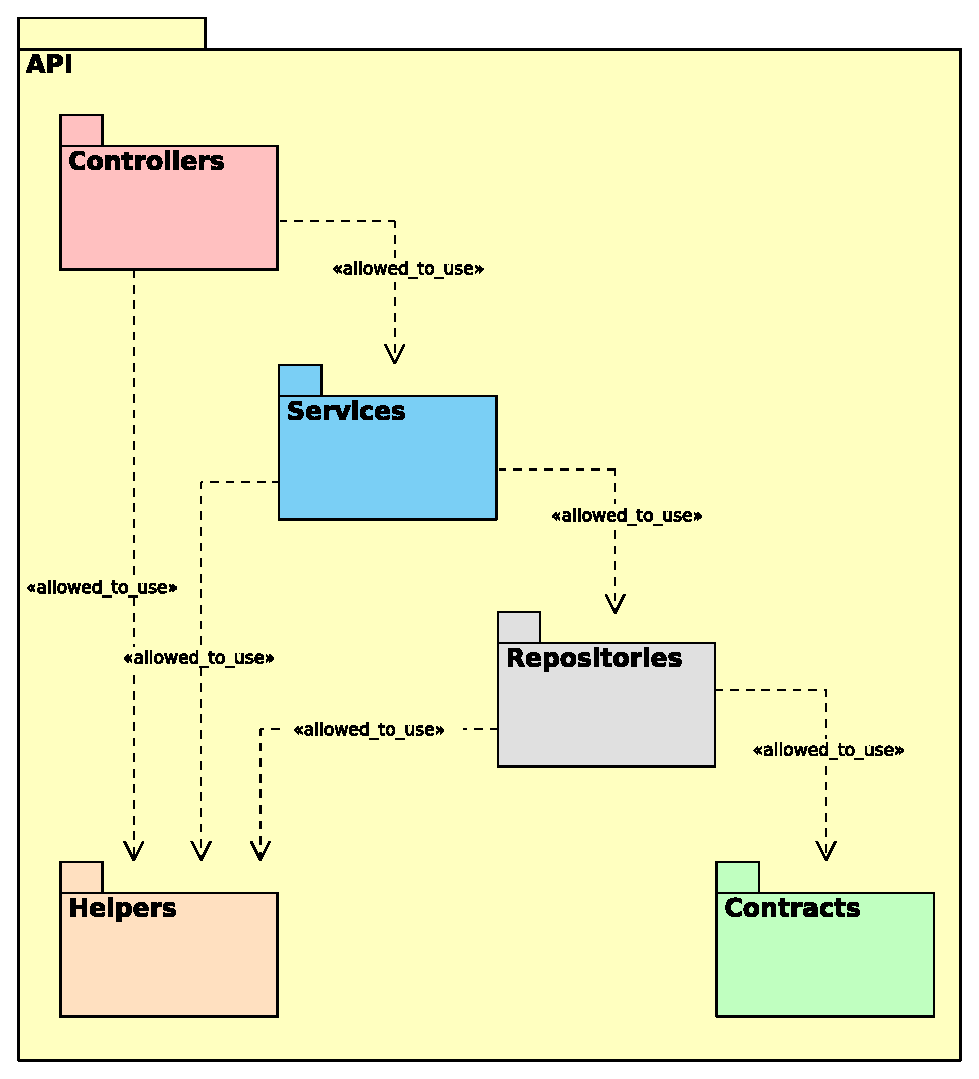
\includegraphics[width=\textwidth]{03-API-Layer.eps}
\caption{API n-tier layered architectural view}
\label{fig3}
\end{figure}

\subsection{Sequences}
\subsubsection{Certifying students}
The Figure~\ref{fig4} shows the flow for certifying a set of students. The University's designated  official, prepares a CSV\footnote{Comma Separated Values} file containing all the students to be certified in certain course. By fulfilling a form (see Figure~\ref{fig5}), the official completes information of the course (i.e. course name, course code, course starting and finishing dates, and hour intensity).

\begin{figure}
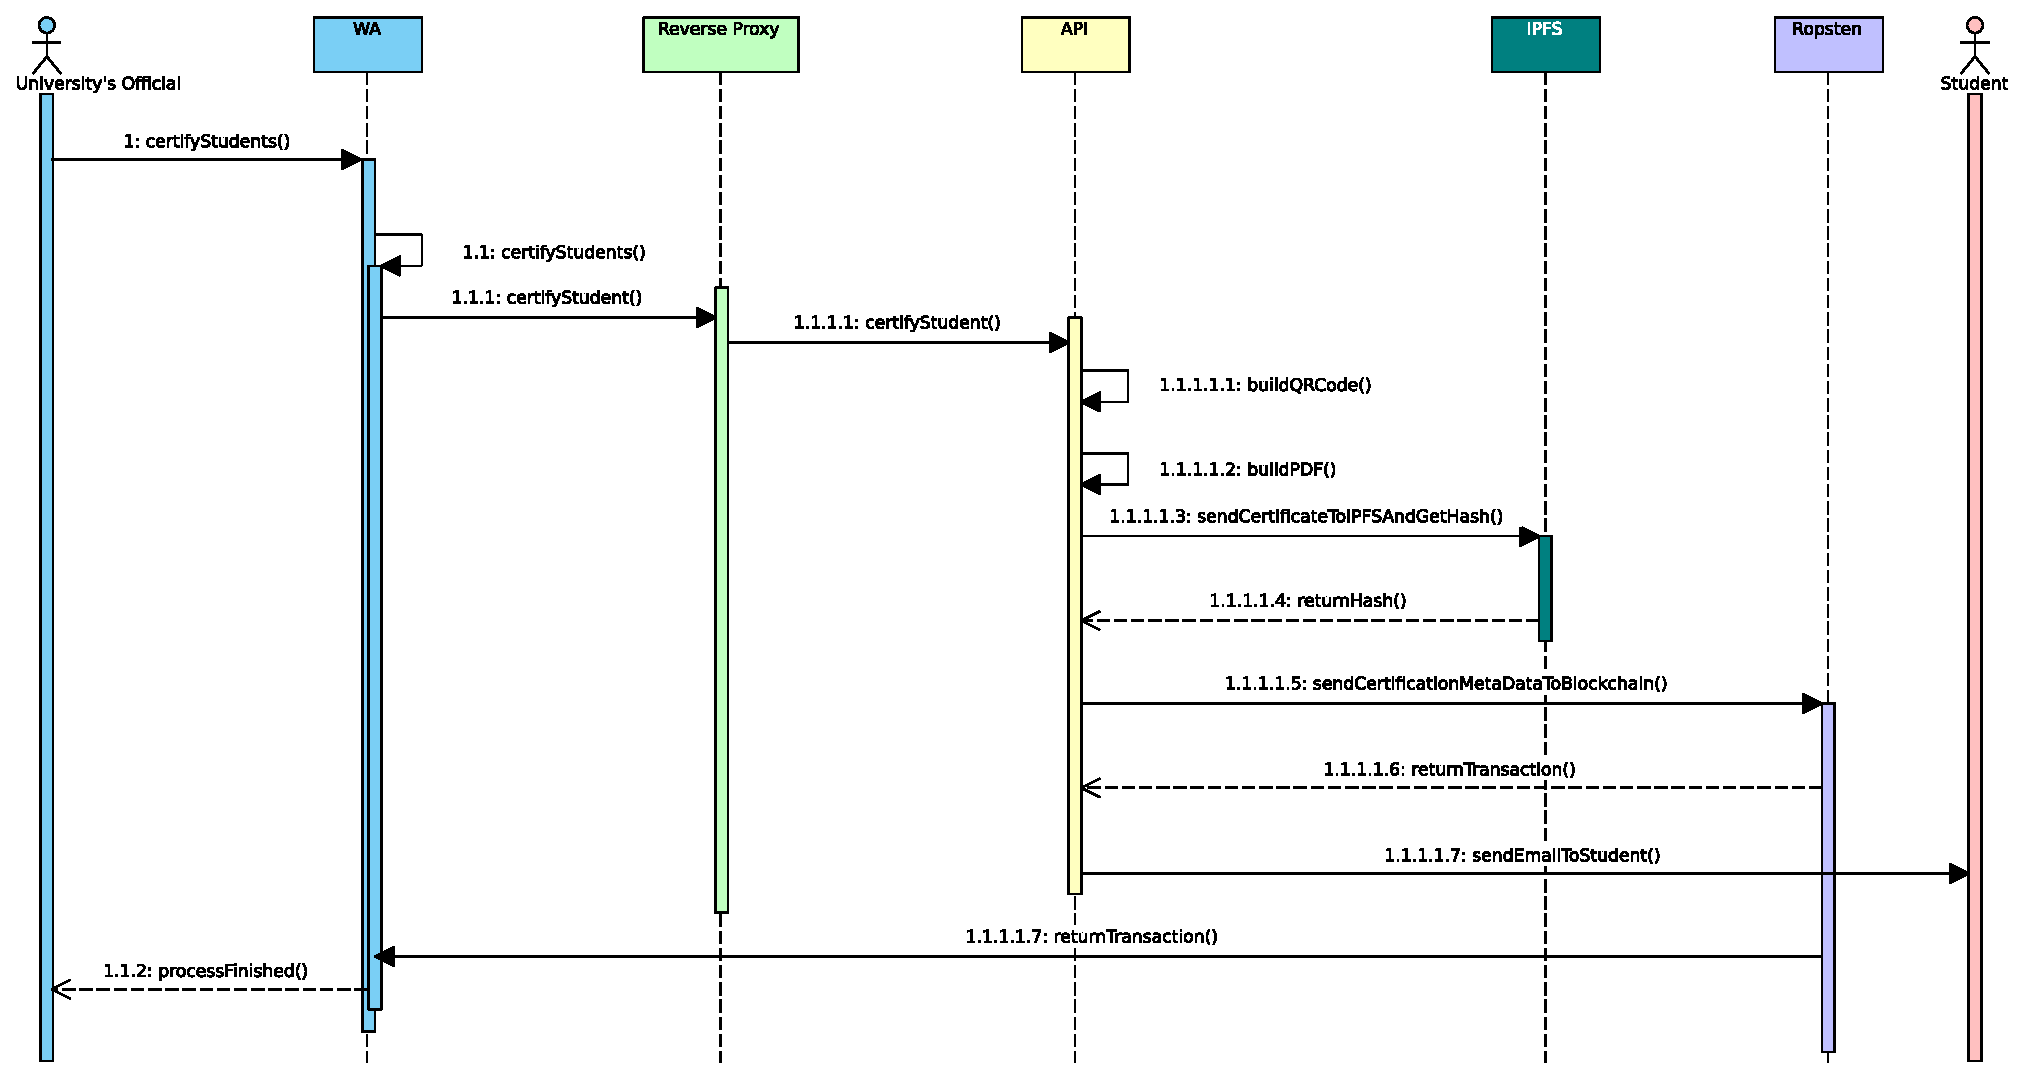
\includegraphics[width=\textwidth]{04-WA-requests-to-API.eps}
\caption{Certifying students sequence diagram.}
\label{fig4}
\end{figure}

\begin{figure}
\includegraphics[width=\textwidth]{05-loader.png}
\caption{WA students loader interface.}
\label{fig5}
\end{figure}

The WA iterates over students, sending a request for certification for each student.

The Reverse Proxy transfer the request to the API, where the data is sanitized, then a unique QRCode is generated in a PNG JS Buffer upon data and a secret salt text. Having the QRCode, the PDF JS Buffer is created upon data and sent to the IPFS network, where the file is going to be hosted, returning its respective hash. The API sends a self signed transaction to the Ropsten network comprised of all the metadata, the IPFS hash and the self generated hash used to create the QRCode. Once the transaction is confirmed, an email is sent to the student with the PDF, its IPFS hash, QRCode and link as attachments.

Parallelly, the WA is listening to the transaction confirmation, once it gets it, starts the process for the next student until the list gets empty.

\subsubsection{Verifying certifications by QRCode} \label{sssec:lbyQrcode}
Verification by QRCode is thought to quick verification with cell phones. It uses the responsive feature of the WA. It's a specific case of sub-sub-section \ref{sssec:lbyLink} (Verifying certifications by link).

\subsubsection{Verifying certifications by link} \label{sssec:lbyLink}
One of the forms to verify the veraciousness of the certificate, is accessing via a link (see Figure~\ref{fig6}). The link has a code that is queryied by the WA to the API through the Reverse Proxy. The API sends the code to the SmartContract. The SmartContract uses an internal structure to save this link code and binds it to the certificate's IPFS hash (see sub-section~\ref{ssec:smartcontract}).

\begin{figure}
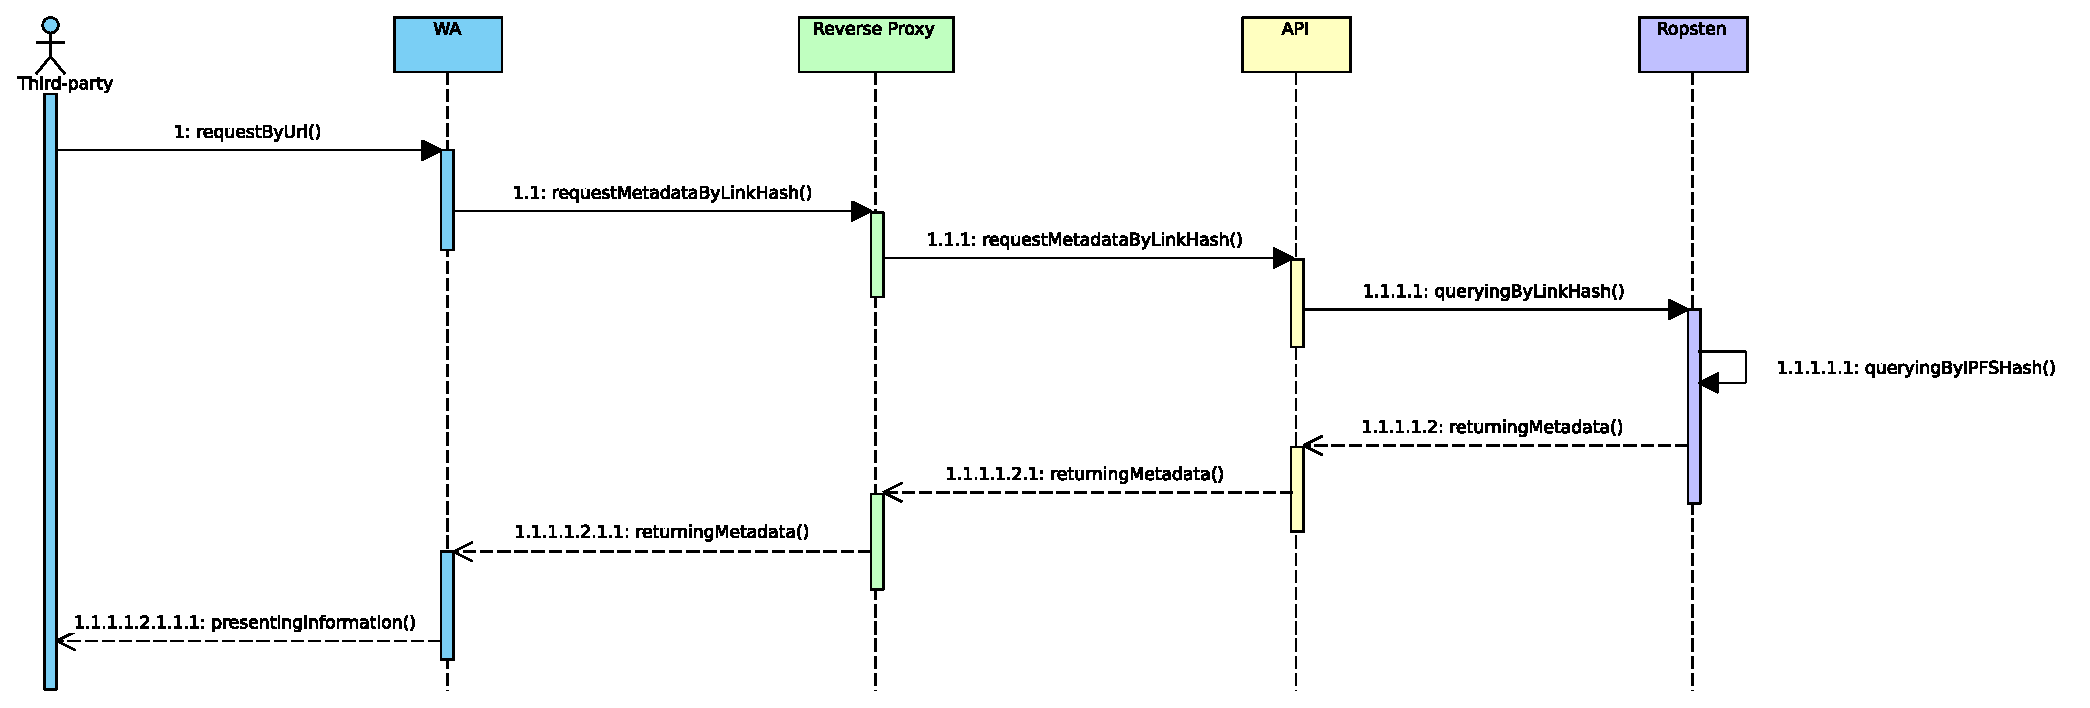
\includegraphics[width=\textwidth]{06-verifying-by-link.eps}
\caption{Verifying certificate information via link.}
\label{fig6}
\end{figure}

\subsubsection{Verifying certifications by PDF} \label{sssec:lbyPDF}
This is the most appealing way to verify authenticity of certificates, because the student can share a copy of their certificate and any third-party can check it through the site.

\begin{figure}
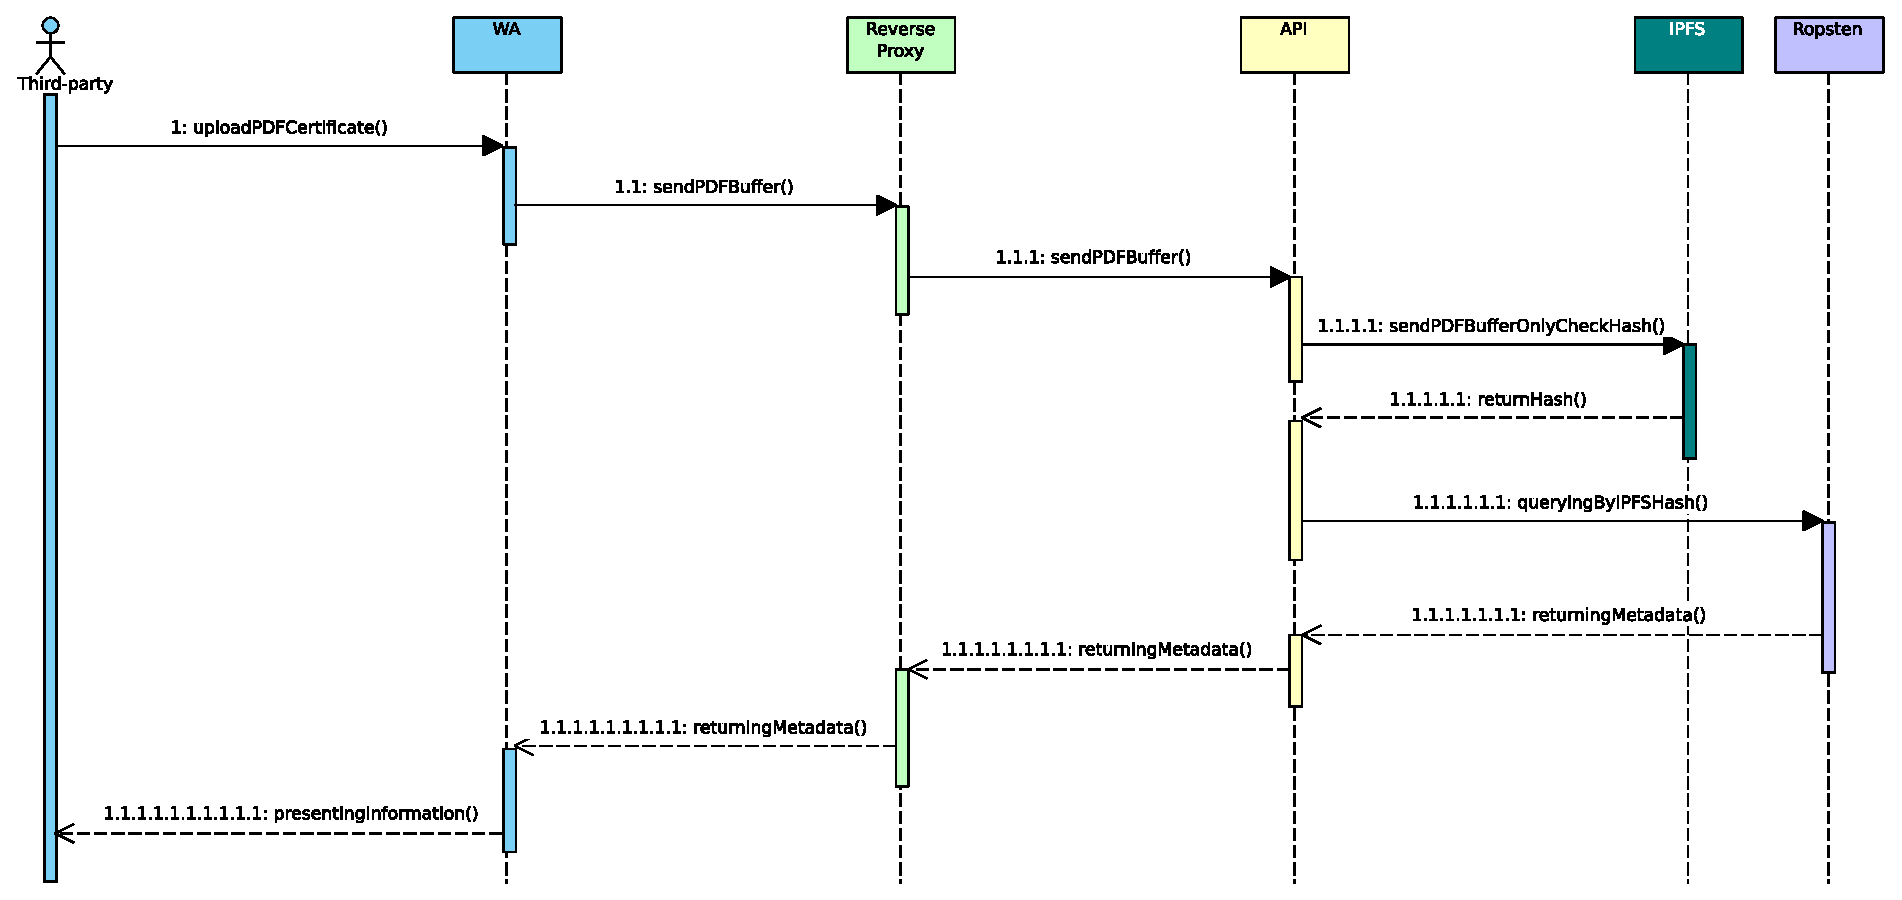
\includegraphics[width=\textwidth]{07-verifying-by-pdf.eps}
\caption{Verifying certificate information via PDF file.}
\label{fig7}
\end{figure}

The third-party will go to \url{https://certificados.bogota.unal.edu.co/} as shown in the Figure~\ref{fig8}, will upload the PDF file (see Figure~\ref{fig7}), it will go to the API through the Reverse Proxy. The API will send the PDF buffer to IPFS but not to add it, but just to get its hash, once it gets the hash it queries the SmartContract with that hash, returning the metadata associated to it, and presented through the WA.

\begin{figure}
\includegraphics[width=\textwidth]{08-home.png}
\caption{Universidad Nacional de Colombia's certificates home.}
\label{fig8}
\end{figure}

\subsubsection{Verifying certificate by hash}
This is a simple way to verify the integrity by the PDF file's hash. This hash is delivered to the student in the notification email. They can provide the hash text to any third-party, who will paste it in the hash section as seen in the Figure~\ref{fig8}. This simply is a simplification of the process shown in the sub-sub-section \ref{sssec:lbyPDF} (Verifying certifications by PDF).

\begin{figure}
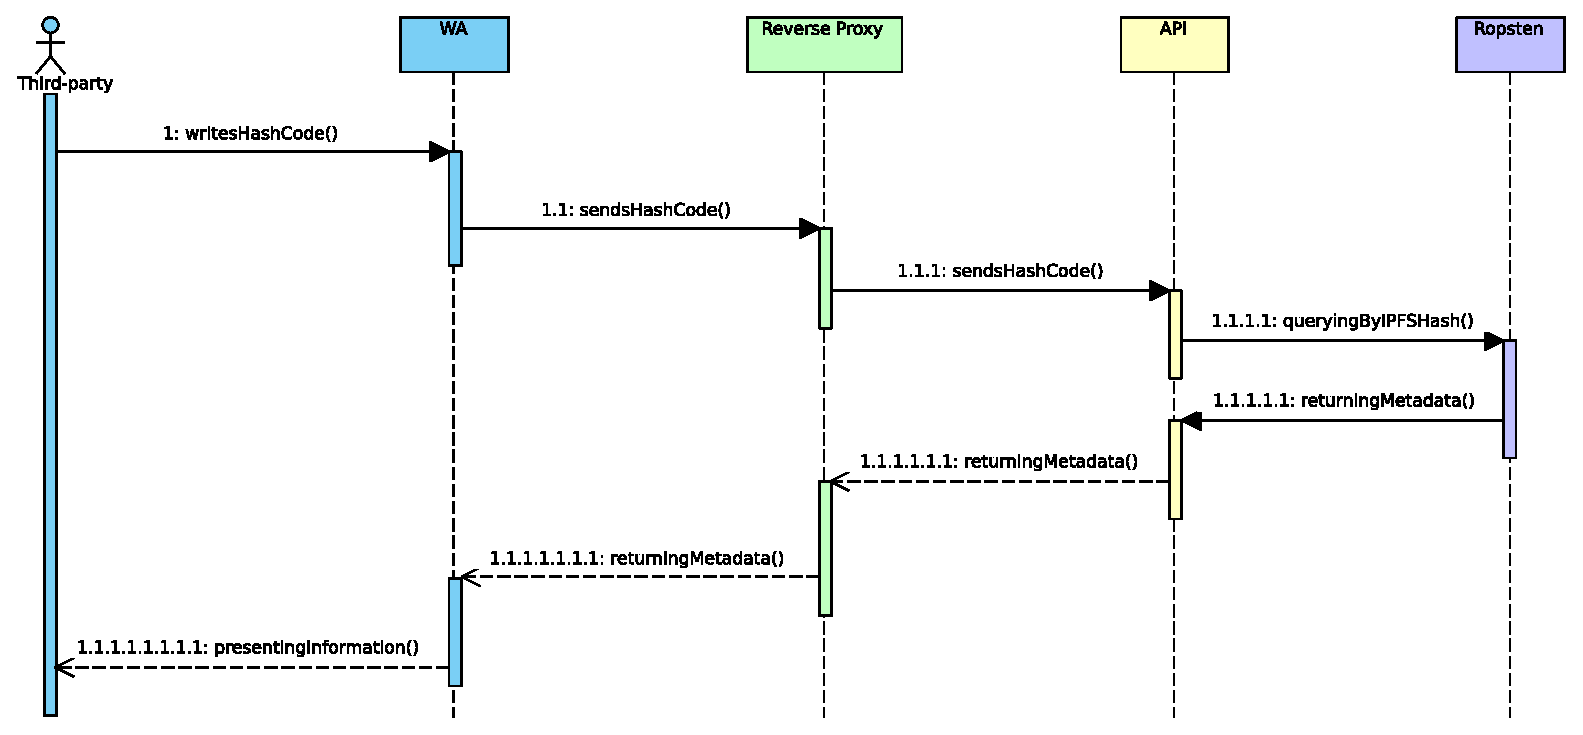
\includegraphics[width=\textwidth]{09-verifying-by-hash.eps}
\caption{Verifying certificate by hash code.}
\label{fig9}
\end{figure}

Once the third-party enters the hash code, this is delivered to the API through the Reverse Proxy, since this is the very hash of the PDF file, there is no need to go to IPFS, the API can query the SmartContract directly.

\subsection{SmartContract} \label{ssec:smartcontract}
SmartContracts are code that encapsulates logic that allows to persist information into the blockchain. They can also read data from the blockchain at the latest known state (other processess might be necessary in order to trace changes in certain data structures as the blockchain constantly changes its final state).

Nevertheless, there is no formal UML representations for what a SmartContract is, but for the sake of explaining the key elements for this project, the Class diagram will fit to show the SmartContract's data structure (see Figure~\ref{fig10}).

\begin{figure}
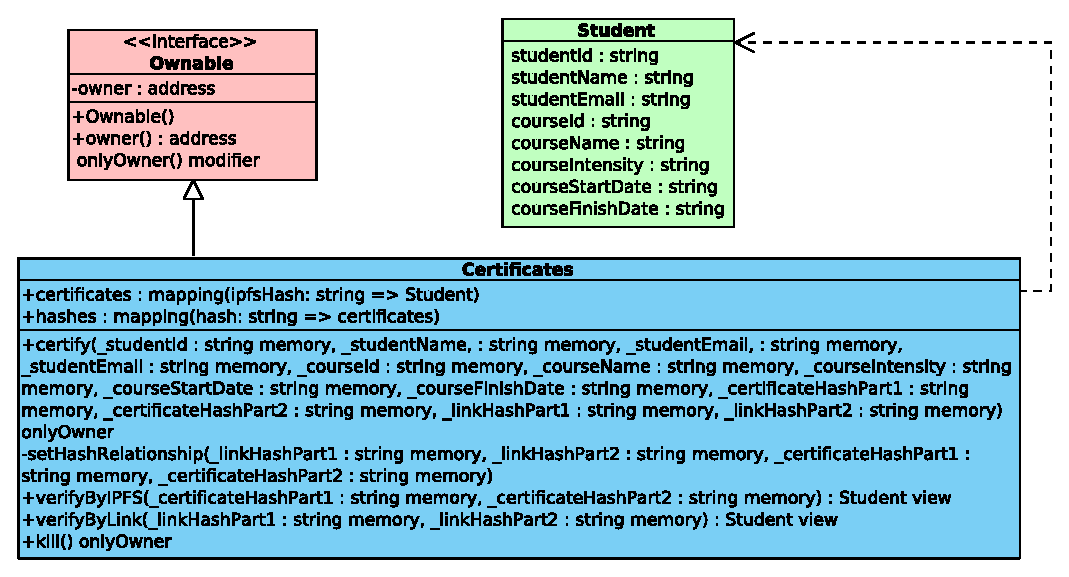
\includegraphics[width=\textwidth]{10-SmartContract.eps}
\caption{SmartContract Class diagram}
\label{fig10}
\end{figure}

The SmartContract has a struct called \emph{Student} as seen on Code~\ref{code:students} (Students struct), to save all the certificate metadata. Such structure is used on the contract in a mapping as shown in the Code~\ref{code:mappings} (SmartContract's mappings).

\begin{Verbatim}[frame=single,numbers=left,label=Students struct]
struct Student {
  string studentId;
  string studentName;
  string studentEmail;
  string courseId;
  string courseName;
  string courseIntensity;
  string courseStartDate;
  string courseFinishDate;
}
\end{Verbatim}
\label{code:students}

\begin{Verbatim}[frame=single,numbers=left,label=SmartContract's mappings]
mapping(bytes32 => mapping(bytes32 => Student)) certificates;
mapping(bytes32 => mapping(bytes32 => string[2])) hashes;
\end{Verbatim}
\label{code:mappings}

The reason to save students within a nested mapping is due to strings in Solidity: they are considered as dynamic-size arrays, and they poses problems not only as key for mappings, but also in response tuples for functions\footnote{This contract was compiled with the pragma 0.4.24. As the documentation states for version 0.5.7, it is now possible to use string as key for mappings (\url{https://solidity.readthedocs.io/en/v0.5.7/types.html\#mappings})}. The IPFS hashes are string of 46 characters length, so a bytes32 data type was not able to hold the hash, making the API to send the IPFS hash in two chunks.

As it was explained before on sub-sub-sections \ref{sssec:lbyQrcode} (Verifying certifications by QRCode) and \ref{sssec:lbyLink} (Verifying certifications by link), it is possible to retrieve the information from the SmartContract using a code. That code reads from the \emph{hashes} mapping, taking the information from the \emph{certificates} mapping as the Code~\ref{code:verification} (Verification Methods) shows.

\begin{Verbatim}[frame=single,numbers=left,label=Verification Methods]
function verifyByIPFS(
    string memory _certificateHashPart1,
    string memory _certificateHashPart2
  ) public view returns (
      string memory,
      string memory,
      string memory,
      string memory, 
      string memory, 
      string memory
    ) {
    bytes32 part1 = _certificateHashPart1.stringToBytes32();
    bytes32 part2 = _certificateHashPart2.stringToBytes32();
    Student memory student = certificates[part1][part2];
    return (
    student.studentId,
    student.studentName,
    student.courseName,
    student.courseIntensity,
    student.courseStartDate,
    student.courseFinishDate
    );
  }

  function verifyByLink(
    string memory _linkHashPart1,
    string memory _linkHashPart2
  ) public view returns (
      string memory,
      string memory, 
      string memory,
      string memory, 
      string memory, 
      string memory
    ) {
    bytes32 part1 = _linkHashPart1.stringToBytes32();
    bytes32 part2 = _linkHashPart2.stringToBytes32();
    string[2] memory IPFSHashes = hashes[part1][part2];
    return verifyByIPFS(IPFSHashes[0], IPFSHashes[1]);
  }
\end{Verbatim}
\label{code:verification}

The way to bind both mappings is shown in the Code~\ref{code:binding} (Mappings binding).

\begin{Verbatim}[frame=single,numbers=left,label=Mappings binding]
function setHashRelationship(
    string memory _linkHashPart1,
    string memory _linkHashPart2,
    string memory _certificateHashPart1,
    string memory _certificateHashPart2
  ) private {
    hashes[_linkHashPart1.stringToBytes32()]
      [_linkHashPart2.stringToBytes32()] = 
      [_certificateHashPart1, _certificateHashPart2];
  }
\end{Verbatim}
\label{code:binding}

Finally, in order to properly query all the certificates of a student an additional information is stored alongside the metadata in the transaction: an event that allows to query by the student id number as the Code~\ref{code:event} shows (Student certified event).

\begin{Verbatim}[frame=single,numbers=left,label=Student certified event]
event studentCertified(
    bytes32 indexed _studentId,
    bytes32 _part1,
    bytes32 _part2
  );
\end{Verbatim}
\label{code:event}

\section{Future work}
Coming work for this project will focus on improving the SmartContract by integrating features on newer versions of Solidity. The contract will be killed after migrating transactions into a Production network. 

%
% ---- Bibliography ----
%
% BibTeX users should specify bibliography style 'splncs04'.
% References will then be sorted and formatted in the correct style.
%
\bibliographystyle{splncs04}
\bibliography{/home/mesi/Documents/BibTex/NLP.bib}
%
%\begin{thebibliography}{8}
%\bibitem{ref_lncs1}
%Author, F., Author, S.: Title of a proceedings paper. In: Editor,
%F., Editor, S. (eds.) CONFERENCE 2016, LNCS, vol. 9999, pp. 1--13.
%Springer, Heidelberg (2016). \doi{10.10007/1234567890}
%\end{thebibliography}
\end{document}
